\chapter{Wprowadzenie}
\thispagestyle{chapterBeginStyle}
\label{rozdzial1}
\section{Planowanie}

    Każdy człowiek wielokrotnie w swoim życiu wykonuje proces określony mianem planowania, często nie zważając na to, jak skomplikowaną pracę wykonuje.
    Skonstruowane przez ludzi plany mogą odnosić się do tak trywialnych zagadnień jak utworzenie listy zakupów, która wprost jest generowana przez braki
    w domowej lodówce oraz upodobania gastronomiczne kupującego, do bardziej abstrakcyjnych form jak \textit{plan na życie}, czy \textit{plan na wygranie meczu}.
    Przyglądając się planom oraz ich własnościom można wyodrębnić następujące trzy aspekty:
    \begin{definition}
    \label{StanyPoczatkowe}
        \textbf{Warunki początkowe} -- stan świata przed rozpoczęciem wykonywania czynności. W dalszej części pracy również określane jako 
        \textbf{stany początkowe}.
    \end{definition}
    \begin{itemize}
        \item Każdy plan musi mieć jasno zadeklarowane warunki początkowe.
        Dzięki dokładnej wiedzy o świecie możliwym jest poprawne określenie akcji, przy pomocy których wprowadzane są modyfikacje
        obecnego stanu aż do otrzymania zadowalających rezultatów. Dla przykładu, firma musi wiedzieć ile oraz jakie palety 
        przybędą na magazyn zanim rozpocznie planowanie rozkładu dostawy na magazynie.
    \end{itemize}
    \begin{definition}
    \label{Akcje}
        \textbf{Akcja} -- działanie zmieniające przedstawiony świat w ściśle określony sposób. W dalszej części pracy również określana jako
        \textbf{operator}.
    \end{definition}
    \begin{itemize}
        \item Akcje pozwalają na modyfikację przedstawionego świata. Każda z akcji składa się \\
        z podmiotu, na który działa oraz czynności,
        która jest względem wskazanego podmiotu wykonywana. Przykładem dobrze określonej akcji może być przeniesienie klocka z 
        jednego stolika na drugi- składa się ona z podmiotu w postaci klocka, oraz czynności w postaci przenoszenia, które możemy traktować
        w ogólniejszy sposób jako ruch. Czynności mogą różnić się od siebie w kwestii skomplikowania, najważniejszym jest, aby były określone poprawnie i aby były wykonalne
        w zdefiniowanym świecie.
    \end{itemize}
    \begin{definition}
    \label{Cel}
        \textbf{Cel} -- Oczekiwany stan świata.
    \end{definition}
    \begin{itemize}
        \item Kwintesencją każdego planu jest cel, który należy uzyskać. Zwyczajowo plany składają się z celów możliwych do
        osiągnięcia ze stanu początkowego przy pomocy zdefiniowany operacji, jednakże trzeba wziąc pod uwagę sytuację, w której 
        niemożliwym jest uzyskanie wskazanego celu, szczególnie próbująć automatyzować pojęcie planowania.
    \end{itemize} 
    Przy pomocy powyższych definicji możliwym jest sformalizowanie pojęcia stojącego za słowem \textbf{plan}. 
    \begin{definition}
    \label{Plan}
    \textbf{Plan} -- lista akcji, której zastosowanie do stanu początkowego powoduje jego zmianę do stanu określonego w ramach celu. 
    \end{definition}

    Oczywiście nie każdy plan musi być wykonalny. Zdarzają się również sytuacje, w których nie da się utworzyć planu dla zadanych warunków 
    początkowych oraz celu. Implementowany algorytm jest w stanie sprawnie poradzić sobie z takimi przypadkami,
    jednakże istnieje inna grupa przypadków, która z persepktywy ów metodologii jest niemożliwa do realizacji. 
    Mowa tu o sytuacjach, gdy któraś z akcji zmienia się w akcję \textbf{warunkową}.
    \begin{definition}
        \label{Akcja warunkowa}
        \textbf{Akcja warunkowa} to typ akcji, która w zależności od bieżącego stanu świata produkuje różne wyniki
    \end{definition}

    Przykładem akcji warunkowej jest kopnięcie dmuchanej piłki. W zależności od wiejącego wiatru, który często zmienia się w sposób dynamiczny, 
    przyłożenie tej samej siły do kopnięcia skutkuje różnym punktem końcowym trasy piłki. Ze względu na ograniczenia języka STRIPS,
    o którym więcej w dalszej części rozdziału, plany w 
    takim kontekście są niemożliwe do utworzenia. Z tej przyczyny wszystkie opisane w ramach badań sytuacje zostaną spreparowane w taki sposób, aby
    były możliwe do całkowitego zrealizowania wykorzystując język akcji STRIPS.
    
    \begin{figure}[H]
        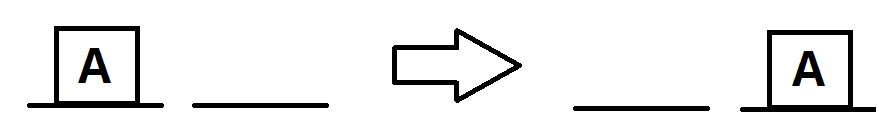
\includegraphics[scale=0.5]{Przyklad1}
        \centering
        \caption{Przeniesienie klocka z jednej półki na drugą jako przykład sytuacji
        dla której istnieje możliwość utworzenia planu. Po lewej stronie od strzałki znajduje się stan
        początkowy, natomiast po prawej- oczekiwany cel. Naturalną akcją w przedstawionym świecie jest akcja \textit{przenieś}, która
        zadany klocek przenosi z jednej półki na drugą.}
        \label{Przyklad1}
    \end{figure}
    Łatwo zauważyć na podstawie przykładu \ref{Przyklad1}, iż można utworzyć wiele planów, które dla zadanego stanu początkowego 
    osiągają wskazany cel. Dla powyższej sytuacji naturalnym planem jest przeniesienie klocka A z platformy po lewej stronie na platformę po prawej stronie, 
    lecz nie jest to jedyna możliwość. Również satysfakcjonującym planem zgodnie\\
    z wprowadzoną wyżej definicją byłaby następująca sekwencja
    akcji:
    \begin{enumerate}
        \item Przenieś klocek A z lewej platformy na prawą
        \item Przenieś klocek A z prawej platformy na lewą
        \item Przenieś klocek A z lewej platformy na prawą
    \end{enumerate}
    Generowanie rekruencyjne nieskończonych planów poprzez bezużyteczne przestawienia \\
    w miejscu, mimo tego, iż zawiera się w definicji \ref{Plan},
    nie jest oczekiwanym efektem. Proces planowania odbywa się po to, by wykonać transformację świata przy jak najmniejszym
    nakładzie sił w jak najkrótszym czasie. Z tego względu wprowadzono pojęcie \textbf{planu optymalnego}.
    \begin{definition}
        \label{PlanOptymalny}
        \textbf{Plan optymalny} -- plan o minimalnej liczbie kroków satysfakcjonujący wskazany cel. 
    \end{definition}
     
    W dalszej części pracy słowo \textbf{plan} najczęściej będzie utożsamiane z planem optymalnym.
    
    Wprowadzenie powyższej definicji wiąże się z powstaniem bardzo ważnego pytania: \\
    \textit{Jak utworzyć plan optymalny?}. Bazując na przykładach
    takich jak \ref{Przyklad1} złudną może być myśl, iż generowanie optymalnych planów jest rzeczą prostą. Niech kolejny przykład będzie tego
    dowodem.
    \begin{figure}[H]
        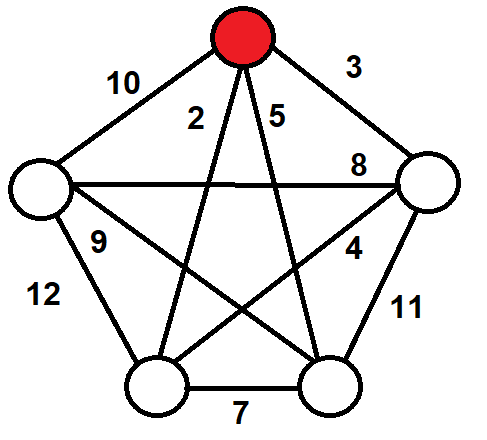
\includegraphics[scale=0.5]{Przyklad2}
        \centering
        \caption{Problem komiwojażera (Travelling Salesman Problem, TSP). Na rysunku pomocniczym liczby symbolizują wagi krawędzi. Węzeł oznaczony
        kolorem czerwonym odpowiada węzłowi startowemu, do którego należy wrócić. Długości krawędzi nie zachowują wskazanych przez wagi proporcji.}
        \label{TSP}
    \end{figure}
    Problem komiwojażera jest popularnym zagadnieniem optymalizacyjnym, którego istotą jest wskazanie ścieżki o najmniejszej sumie wag krawędzi, 
    która przechodzi dokładnie jeden raz przez każdy wierzchołek i wraca do wierzchołka startowego. Często problem wędrującego 
    komiwojażera przedstawiany jest przy pomocy kuriera oraz domów, które musi odwiedzić\\
    (za wierzchołek startowy uważa się magazyn,
    w którym kurier rozpoczyna swoją pracę). Mimo faktu, iż w przykładzie \ref{TSP} występuje jedynie 5 miejsc, 
    w których musi zatrzymać się kurier, utworzenie optymalnego planu dla przedstawionej sytuacji okazuje się być prawdziwym wyzwaniem. Z tego powodu 
    ludzie postanowili skorzystać z mocy obliczeniowych komputerów przy generowaniu bardziej skomplikowanych planów, w celu zapewnienia ich 
    optymalności.


\section{Planowanie przy użyciu komputerów}

    \subsection{STRIPS}
    \label{STRIPSRozdział}
    W 1971 roku Panowie: Richard Fikes oraz Nils Nillson z Standford Research Institute (SRI International, 
    jeden z najsłynniejszych na świecie ośrodków badawczych) zdecydowali się na przedstawienie światu
    nowego podejścia w dziedzinie planowania o nazwie \textbf{STRIPS} (\textbf{ST}anford \textbf{R}esearch \textbf{I}nstitute
    \textbf{P}roblem \textbf{S}olver)\cite{STRIPS}.
    \textbf{STRIPS} rozwiązuje wskazany problem poprzez przeszukiwanie wszystkich stanów świata, aż do momentu
    gdy znajdzie taki, w którym wskazane cele są spełnione. Ważnym założeniem programu jest istnienie
    ciągu akcji, który gwarantuje otrzymanie celu. Zadanie to jest realizowane poprzez znalezienie
    sekwencji operatorów, która konwertuje wymodelowany stan początkowy w model, w którym wszystkie 
    zdefiniowane cele są spełnione. Defnicje operatorów, stanu początkowego oraz celu\\
     są niemalże identyczne jak 
    \ref{StanyPoczatkowe}, \ref{Akcje} i \ref{Cel}, z tym, że definicja akcji została w naturalny sposób rozwinięta o ciąg przyczynowo-skutkowy. Zauważono, iż w skład każdej akcji 
    poza samą czynnością wchodzą dwie składowe, nazywane środowiskowymi- warunki zajścia oraz efekty zajścia. 
    \begin{definition}
        \label{WarunekAkcji}
        \textbf{Warunkiem} zajścia akcji jest istnienie odpowiedniej konfiguracji świata, dzięki której akcja może zostać wykonana.
    \end{definition}
    \begin{definition}
        \label{EfektAkcji}
        \textbf{Efektem} zajścia akcji są zmiany, które zaszły w przedstawionym świecie \\
        ze względu na jej wykonanie.
    \end{definition}
    Reasumując, każda akcja ma swoją przyczynę oraz swój skutek. \textbf{Przyczyną} akcji w przykładzie \ref{Przyklad1} jest znajdowanie się klocka na lewej platformie. Gdyby
    klocek A znajdował się na prawej platformie, wykonanie akcji przesunięcia klocka z platformy lewej na prawą byłoby niemożliwe do wykonania, natomiast \textbf{efektem} akcji jest 
    przeniesienie klocka na prawą platformę. Łatwo zauważyć, iż brak innych obiektów na platformie prawej jest niezbędny, aby klocek mógł zostać tam przeniesiony.
    Jeśli na platformie prawej znajdowałby się inny klocek o sygnaturze \texttt{B}, wtedy przesunięcie klocka \texttt{A} odbyłoby się bezpośrednio na 
    bloczek B \\ 
    a nie na samą platformę. W takim przypadku, o fakcie pobytu klocka A na prawej platformie algorytm dowiedziałby się poprzez przechodniość 
    relacji pobytu.

    Kolejną naturalną obserwacją jest stwierdzenie, iż przeprowadzenie akcji dodaje nam nowe informacje o świecie w dwóch kontekstach:
    \begin{itemize}
        \item Dodającym -- pojawienie się lub podtrzymanie danej składowej świata
        \item Usuwającym -- pozbawienie świata danej składowej
    \end{itemize}
    Po wykonaniu czynności z przykładu \ref{Przyklad1} wyróżniono trzy typy informacji:
    \begin{itemize}
        \item Warunek- Obecność klocka na lewej platformie, prawa platforma jest pusta
        \item Efekt dodający -- Obecność klocka na prawej platformie
        \item Efekt usuwający -- Brak obecności klocka na lewej platformie (platforma lewa jest pusta)
    \end{itemize}
    W rozważanym podejściu każda z czynności zdefiniowana jest przy pomocy wyżej wskazanych trzech składowych.

        Takie zdefiniowane świata okazuje się wystarczające do rozwiązywania problemów pokroju rearanżacji obiektów czy 
    nawigowania w ściśle zdefiniowanej przestrzeni, czego najlepszym przykładem, jest pierwszy robot do realizacji ów zadań- \textbf{Shakey}.
    Shakey dzięki zainstalowanemu oprogramowaniu,
    posiadał umiejętność analizy własnego otoczenia. Dzięki zaimplementowanemu podejściu 
    STRIPS (oczywiście z odpowiednimi dostosowaniami do sytuacji) był w stanie rozwiązywać problemy z zakresu wyznaczania drogi,
    czy planowania rozmieszczenia obiektów w pokojach.
    Ze względu na swoją innowacyjność i przełomowość często jest nazywany archetypem
    dzisiejszych autonomicznych samochodów czy militarnych dronów.

    Dzięki swojej roli w rozwoju planowania z użyciem komputerów, STRIPS został dodatkowo wyróżniony- od jego nazwy pochodzi język opisu świata korzystający
    z trójki: stan początkowy, akcja oraz cel. Przez następne lata rozwiązania w obszarze planowania silnie bazowały na wprowadzonym w powyższej pracy opisie świata.

    \subsection{Rozwiązywanie ludzkich problemów}
    W 1972 roku Allen Newell i Herbet Simon opublikowali książkę pod nazwą \textbf{Human Problem Solving}, której tłumaczenie
    znajduje się w tytule opisywanej sekcji. Założenie, odnośnie otrzymywanych przez algorytm danych, 
    pozostało zgodne z opisem w sekcji \ref{STRIPSRozdział}, jednakże autorzy pracy zauważyli, iż utworzony w ten sposób 
    obszar działań (\textit{problem space}) może osiągać niebotyczne rozmiary. Chcąc odpowiedzieć na pytanie, 
    w jaki sposób ludzie wybierają odpowiednie operacje w danej sytuacji, zauważyli, iż często wykorzystują oni \textit{skróty},
    które wynikają bezpośrednio z intuicji. Człowiek ze względu na swoją naturę będzie dążył do zużycia jak najmniejszych 
    pokładów energii w celu osiągnięcia wyznaczonego celu. \\ 
    Na tej podstawie rozpoczęło się formowanie 
    technik rozwiązywania problemów zwanych \textbf{heurystykami}. Początkowe heurtystki ograniczały się do zastosowania 
    pewnych ograniczeń jeśli chodzi o wyznaczanie zbioru operatorów, na przykład poprzez unikanie powtórzeń (\textit{repeat-state avoidance})
    oraz unikanie powrotów do stanów już znanych (\textit{backup avoidance}). \\
    Na przestrzeni następnych lat pojęcie heurystyki rozwinie się diametralnie, jednakże
    zachowa swoją pierwotną definicję szukania niekoniecznie najlepszych rozwiązań w zamian za znaczne przyśpieszenie otrzymywanych wyników.

    \subsection{Liniowy i częściowy porządek}
    Na początku lat 70 ubiegłego wieku do tworzenia prostych planów wykorzystywano również pojęcie 
    liniowego porządku (\textit{total order}) sekwencji akcji. W tym podejściu, ochrzczonym mianem \textbf{planowanie liniowe}
    (\textit{linear planning}) dla każdego z celów  próbowano utworzyć odpowiedni podplan, który go osiągał.
    Następnie ów plan łączono przy pomocy odpowiedniego porządku akcji w jeden spójny plan.
    Ze względu na wady tego podejścia, jak długi czas formowania planu oraz możliwość wystąpienia konfliktów między 
    odpowiednimi celami planu, co na początku nie było takie oczywiste, zamiast liniowego porządku zaczęto wykorzystywać porządek częściowy (\textit{partial order}),
    którego przykładem jest omawiany \textbf{GRAPHPLAN}.

    \subsection{ADL i PDDL}
    Action Description Language (w skrócie \textbf{ADL}) zostało zaproponowane przez Edwina Pednault'a  w 1987 roku jako usprawnienie 
    języka opisu STRIPS. Ów system automatycznego planowania został zaprojektowany z myślą o przyszłej implementacji w nowoczesnych na tamten czas robotach.
    Główną ideą stojącą za utworzeniem tego języka opisu problemów było zauważenie, iż język STRIPS nie potrafi poradzić sobie z sytuacjami, gdy
    powstanie danego efektu zależy od istniejących w świecie warunków. Dodatkowym aspektem, którego wprowadzenie znacznie poprawiło wydajność metodologii ADL względem STRIPS 
    było wykorzystanie zasady \textbf{otwartego świata}, która mówi, iż rzeczy nieokreślone w świecie są uznawane jako \textit{nieznane}, a nie jako 
    fałszywe, jak to było w STRIPS, który został stworzony wedle \textbf{zasady zamkniętego świata}. Dodatkowo, ostateczne cele w języku STRIPS mogły być jedynie przedstawione jako 
    koniunkcje stanów (Przykład: Dobra i Tania w kontekście restauracji), czyli jako cele bezwarunkowe. 
    W nomenklaturze ADL cele można przedstawiać również przy pomocy alternatyw, to znaczy: 
    nie wszystkie stany muszą być spełnione, mogły istnieć grupy stanów, w których spełnienie tylko jednego było wystarczające (Przykład: Dobra i (Tania lub Blisko)). 

    Planning Domain Definition Language (w skrócie \textbf{PDDL}) było próbą ustandaryzowania języków wykorzystywanych 
    do planowania przy pomocy komputerów silnie inspirowaną przez swoich poprzedników- STRIPS i ADL. 
    Utworzeniem takiego standardu zajął się Drew McDermott wraz ze współpracownikami z \textbf{Yale University}.
    Podstawową ideą stojąca \\
    za PDDL jest całkowite odseparowanie metod rozwiązywania problemów od środowisk, \\
    w których się 
    znajdują. Techniki rozwiązywania problemów związanych z logistyką (ustalanie najkrótszej drogi) powinny być również aplikowalne do rozwiązywania problemów 
    związanych z produkcją (minimalizacja zużycia materiału). Pozostałe aspekty są porównywalne do języka STRIPS- 
    istnienie warunków początkowych, zbioru operatorów oraz zbioru złożonego z celów do osiągnięcia.



    \subsection{Nowoczesne rozwiązania}
    Wraz z prężnym rozwojem informatyki, dziedzina planowania przy użyciu komputerów również zaopatrzyła się 
    w nowy arsenał, mający na celu usprawnienie jak i ułatwienie generowania planów.
    Pojawiło się wiele innowacyjnych metod, które znacznie wykraczają poza ograniczenia, jakie 
    nakłada język opisu świata STRIPS. Zaczęły powstawać nowe sposoby planowania takie jak planowanie preferencyjne, którego celem jest nie tylko
    utworzenie planu, ale również zapewnienie zachowania preferencji wskazanych obiektów świata. Często taki typ planowania 
    może być wykorzystywany w sytuacjach, które obejmują ludzi, chociażby plan lekcji w szkole i preferencje nauczycieli odnośnie godzin pracy.
    Ponadto zaistniał diamentralny rozwój w programowaniu warunkowym, który może reagować na nieznane 
    czynniki przedstawionego świata. Pozwala to na redukcję obszaru poszukiwań na kawałki,co sprowadza 
    się do łatwiejszego przedstawiania złożonych problemów oraz uzyskiwania szybszych wyników przez algorytmy implementujące podejście 
    warunkowe. Poza rozwojem opisu dopuszczalnych akcji, dokonano również rozbudowy opisu stanów w świecie.
    Dla przykładu, \textbf{algorytmy online} charakteryzują się tym, iż są w stanie generować plany mimo braku posiadania całkowitej 
    wiedzy o świecie w momencie rozpoczęcia pracy. Do algorytmu dane przekazywane są partiami. Na podstawie przesłanych informacji algorytm dokonuje 
    odpowiednich decyzji i udziela odpowiedzi. Proces kontynuowany jest aż do momentu przetworzenia wszystkich wprowadzonych danych. Sztandarowym 
    wykorzystaniem algorytmów online jest mechanizm przydzielania pamięci procesa do procesów w komputerze.

    
    \subsection{Miejsce GRAPHPLAN'u}
    Między powstaniem metodologii STRIPS a jej rozszerzeniami w postaci ADL lub PDDL powstawały również inne podejścia, w tym silnie 
    bazujący na grafach, własnościach częściowego porządku i ich możliwościach, algorytm o wdzięcznej nazwie \textbf{GRAPHPLAN}.






